\chapter{Chapter Four}
\section{Discussion}
It has been shown that the constrained $Z_{DR}$ datasets aid in determining event biases, which then allows hydrometeor type to be inferred from the unbiased
datasets. Now, statistics are compiled, and the probable source of the \hl{inferred bias} addressed. The relative merit of the two radar systems in observing lake-effect
snow is also discussed.
\subsection{Diagnosing Inferred $Z_{DR}$ Bias}
The source of the \hl{inferred observational bias at CWKR} could be due to large differences in beam volumes between radars, in combination with a large gradients of $Z_{DR}$ with height. A similiar result was found by \citep{Ryzhkov2007a}, in that cross-beam gradients of $Z_{DR}$ can produce significant biases. Modeling the beam as a Gaussian function, Equation \ref{eq:beam_pattern} gives the solid angle of the beam, as a function of beamwidth $\theta$ \citep{Probert1962}. 
\begin{equation}\label{eq:beam_pattern}
\Omega = \int \int f^{2}(\theta) d\omega \approx \frac{\pi \theta^{2}}{8 \ln 2}
\end{equation}
\begin{equation}\label{eq:beam_volume}
V = \frac{\Omega}{4\pi} * \frac{4}{3} \pi r^{3}
\end{equation}
 Equation \ref{eq:beam_volume} describes how the \hl{theoretical beam volume} broadens as range ($r$) increases. \hl{The theoretical beam volume is modeled as a spheroid, and is an average over a window of pulse volumes.} This combined with 
 differing $\Omega$ creates the large difference in beam volumes between radars, as shown in Figure \ref{fig:ideal_beam}.
\begin{figure}[H]
\centering
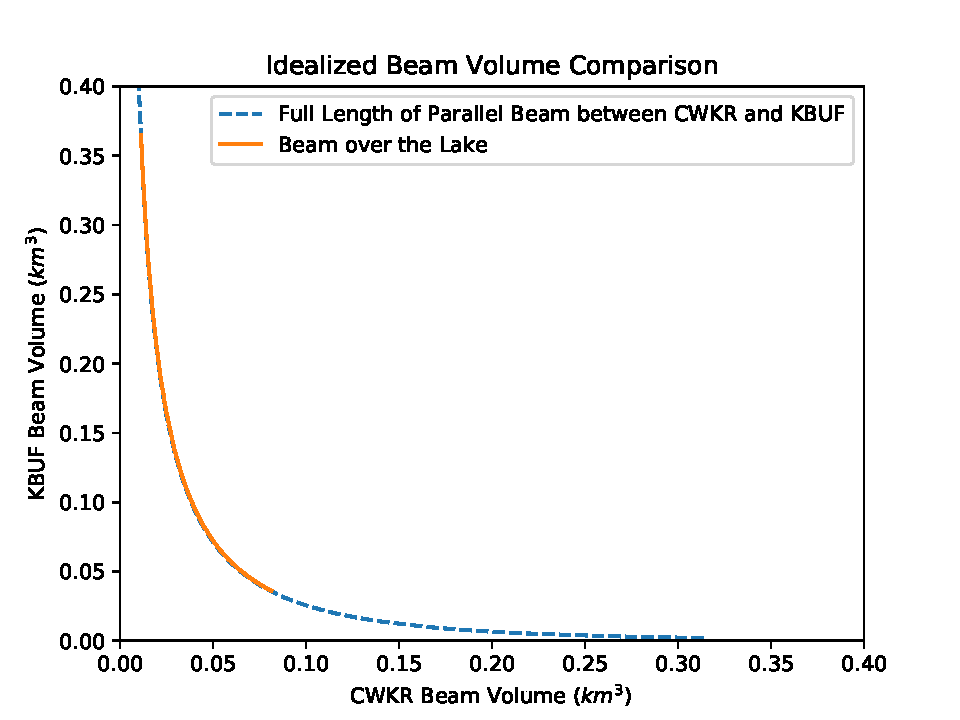
\includegraphics[width=\textwidth]{ideal_beam}
\caption{Gate-by-gate idealized beam volume comparison along a straight line between radars, assuming Gaussian beam functions.} 
\label{fig:ideal_beam}
\end{figure}
 As to why only certain cases are biased, it is likely due to these cases containing deeper, more intense 
 precipitation, with more opportunity for intra-cloud variations, e.g. ongoing aggregation. As shown in Table \ref{diagnosebias}, biased cases contain precipitating structures that are on average 1.1 km deeper than unbiased threshold
 cases. Furthermore, biased cases are shown to be more intense, with average $Z_{eH}$ values 2-3 dBZ greater 
 than unbiased cases. This difference is significant as it falls beyond the standard error of the two means. 
Another result that supports this is found by comparing the range of $Z_{DR}$ values present in each case. As 
shown in Figure \ref{fig:bias_range}, the biased cases tend towards a larger range of values than unbiased. 
\begin{table}[H]
    \caption{Comparing depth and intensity of unbiased and biased cases, where the overbar indicate global means.}\label{diagnosebias}
    \begin{center}
    \begin{tabular}{|l|c|c|c|}
    \hline
    \multicolumn{4}{|c|}{Unbiased Cases} \\
    \hline
     Event & Echo Top (km) & CWKR $\overline{Z_{eH}}$ (dBZ) & KBUF $\overline{Z_{eH}}$ (dBZ)\\
    \hline\hline
    2014-01-18 & 2.4 & 10 & 11 \\
    \hline
    2014-01-23 & 1.9 & 14 & 14 \\
    \hline
    2015-01-06 & 0.5 & 11 & 8 \\
    \hline
    2015-01-07 & 3.2 & 18 & 17 \\ 
    \hline
    2016-02-10 & 1.9 & 12 & 15 \\ 
    \hline\hline
    Mean & 2.0 & 13 & 13 \\
    \hline
    \hl{Standard Error} & 0.20 & 0.63 & 0.71 \\
    \hline
    \multicolumn{4}{|c|}{Biased Cases} \\
    \hline\hline
    2014-02-01 & 4.3 & 17 & 18\\
    \hline
    2015-02-06 & 3.9 & 19 & 16\\
    \hline
    2015-02-14 & 2.1 & 14 & 11\\
    \hline
    2015-02-18 & 1.9 & 17 & 16\\ 
    \hline
    2016-12-15 & 3.5 & 13 & 14  \\ 
    \hline\hline
    Mean & 3.1 & 16 & 15 \\
    \hline
    \hl{Standard Error} & 0.22 & 0.49 & 0.53 \\
    \hline
    \end{tabular}
    \end{center}
\end{table}

\begin{figure}[H]
\centering
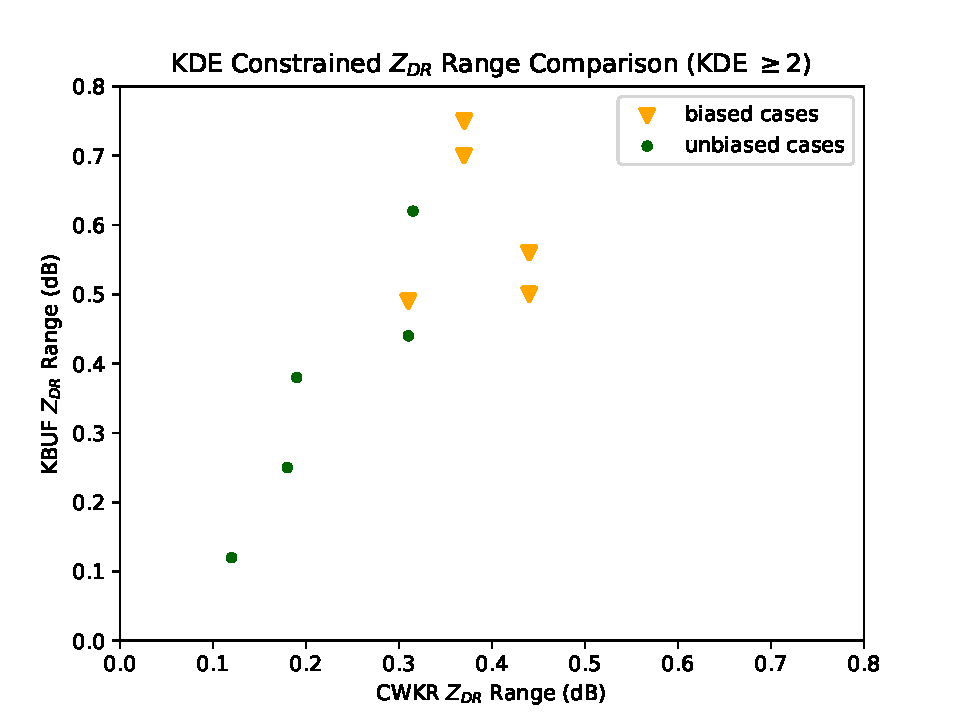
\includegraphics[width=\textwidth]{bias_range}
\caption{Comparison of the range of $Z_{DR}$ (max-min) values observed for each case.} 
\label{fig:bias_range}
\end{figure}
\subsection{$Z_{DR}$ Statistics}
A statistical comparison of synoptic and lake-effect cases is made in Table \ref{eventcompare}. Both types of events show very similiar mean values, with both radars indicating 0.2 dB for lake-effect and 0.3 dB for synoptic. This suggests that synoptic events tend more towards pristine snow crystals, while lake-effect events contain more aggregated snow. While the mean values match between radars, it is shown that KBUF yields a larger range of $Z_{DR}$ regardless of the type of event. A wider beamwidth could aid in the detection a larger variety of hydrometeor types.
\begin{table}[H]
    \caption{\hl{Bias-adjusted $Z_{DR}$ Statistics, comparing synoptic and lake-effect events. The observational bias between radars as inferred at CWKR is italicized, while the measured hardware bias at KBUF is in bold face.}}\label{eventcompare}
    \begin{center}
    \begin{tabular}{|l|c|c|c|c|c|c|c|c|c|c|}
    \hline 
    \multicolumn{11}{|c|}{Synoptic Events} \\
    \hline
     &
    \multicolumn{5}{|c|}{CWKR $Z_{DR}$ (dB)} & 
    \multicolumn{5}{|c|}{KBUF $Z_{DR}$ (dB)} \\
    \hline 
     Event & \textit{Bias} & Min & Mean & Max & Range & \textbf{Bias} & Min & Mean & Max & Range\\
    \hline\hline
    2014-01-18 & \textit{-0.10} & 0.1 & 0.3 & 0.6 & 0.5 & \textbf{-0.40} & 0.1 & 0.4 & 0.6 & 0.5 \\
    \hline
    2014-02-01 & \textit{0.22} & 0.1 & 0.2 & 0.4 & 0.3 & \textbf{-0.20} & 0.3 & 0.4 & 0.4 & 0.1 \\    
    \hline
    2015-01-07 & \textit{-0.04} & 0.1 & 0.3 & 0.4 & 0.3 & \textbf{-0.30} & 0.0 & 0.3 & 0.4 & 0.4 \\ 
    \hline
    2015-02-06 & \textit{0.28} & 0.0 & 0.1 & 0.3 & 0.3 & \textbf{0.00} & -0.1 & 0.1 & 0.3 & 0.4\\
    \hline
    2016-12-15 & \textit{-0.47} & 0.2 & 0.4 & 0.6 & 0.4 & \textbf{-0.28} & 0.2 & 0.4 & 0.6 & 0.4  \\ 
    \hline 
    Mean  & -- & 0.1 & 0.3 & 0.5 & 0.4 & -- & 0.1 & 0.3 & 0.5 & 0.4 \\
    \hline
    \multicolumn{11}{|c|}{Lake-Effect Events} \\
    \hline\hline
    2014-01-23 & \textit{-0.06} & 0.0 & 0.3 & 0.6 & 0.6 & \textbf{-0.40} & 0.0 & 0.5 & 0.6 & 0.6\\
    \hline
    2015-01-06 & \textit{0.00} & 0.2 & 0.5 & 0.9 & 0.7 & \textbf{-0.10} & -0.1 & 0.5 & 0.9 & 1.0 \\
    \hline
    2015-02-14 & \textit{0.38} & -0.1 & 0.1 & 0.4 & 0.5 & \textbf{-0.10} & -0.1 & 0.1 & 0.4 & 0.5 \\
    \hline
    2015-02-18 & \textit{0.30} & 0.1 & 0.3 & 0.6 & 0.5 & \textbf{-0.10} & -0.1 & 0.4 & 0.6 & 0.7 \\ 
    \hline
    2016-02-10 & \textit{-0.04} & -0.1 & 0.2 & 0.5 & 0.6 & \textbf{0.40} & -0.1 & 0.1 & 0.5 & 0.6  \\ 
    \hline\hline
    Mean & -- & 0.0 & 0.3 & 0.6 & 0.6 & -- & -0.1 & 0.3 & 0.6 & 0.7 \\
    \hline
    \end{tabular}
    \end{center}
\end{table}

\subsection{Relative Merits of C-Band vs. S-Band in Lake-Effect Snow}
The results have shown that the wider beamwidth of S-Band may contribute to the detection of a higher diversity of hydrometeors per sampling volume. This
becomes more critical for mixed phases of precipitation, but for pure snow is not as relevant. For quantitative precipitation purposes this becomes more
relevant, as the shape of the snow crystals can give insights into their density, providing a better estimate of snow-to-liquid ratios. Furthermore,
comparing values of $Z_{eH}$ in lake-effect snow events versus synoptic events has shown that C-Band radar has a slight advantage in detecting shallow snow-squalls.

